\subsection{Figuras}

\subsubsection{Referencia de figuras}

En el reporte pueden utilizarse fotografías, diagramas, gráficas, etc., para mostrar de manera visual información que facilite al lector el entendimiento de la práctica desarrollada. Existen
puntos importantes que deben ser considerados al momento de incluir una imagen, entre los cuales
se enumeran a continuación:

\begin{enumerate}
\item Cada figura que es incluida debe incluir un título y una numeración
\item Cada figura que es incluida debe ser citada en el texto para explicarla
\end{enumerate}

Por ejemplo:

\begin{figure}[!htbp]
        \centering
        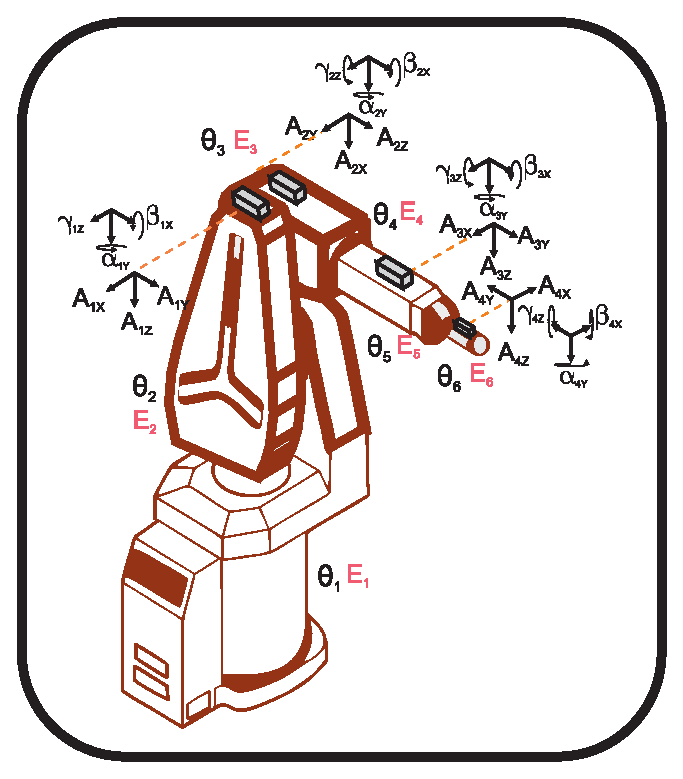
\includegraphics[width=0.4\textwidth]{images/robot.eps}
        \caption{\footnotesize{Variables cinemáticas de un manipulador robótico}}
        \label{fig1_100}
\end{figure}

\emph{
En la figura \ref{fig1_100} se muestran las diferentes variables que se pueden extraer de un manipulador robótico. Para cada uno de los eslabones es posible obtener tres variables de aceleración $A_z$,$A_y$ y $A_z$, 3 variables de velocidad angular, $\alpha$,$\beta$ y $\gamma$,  y una señal de encoder $E$. Es decir, el comportamiento
del eslabón de un manipulador robótico puede extraerse de  7 variables que se relacionan mediante
funciones de integración y derivación (posición-velocidad-aceleración).
}

Como se observa en el párrafo se hace una cita de la imagen \ref{fig1_100}, y también en este se hace una descripción de la información visual más relevante de la imagen, relacionando de esta manera la imagen incluida en el reporte y el texto.


Cuando se agrega una gran cantidad de imágenes relacionadas a un mismo texto a manera de evidencia, no es necesario una explicación tan detallada, una explicación puede abarcar diferentes imágenes, por ejemplo, basta decir que las figuras \ref{fig1_100}, \ref{fig1_101}, \ref{fig1_102}, \ref{fig1_103} y \ref{fig1_107}, han sido incluidas para llevar a cabo demostraciones de lo que se explica en esta guía.

\subsubsection{Fotografías}

Las imágenes que se utilizan en un reporte son usualmente fotografías evidencia del proyecto realizado. En este caso es indispensable que las fotografías tomadas sean nítidas y centren
de manera visual las características que se quieren resaltar.

En ocasiones será necesario editar las fotografías para resaltar elementos o características que puede desconocer el lector. Por ejemplo:

\emph{En la figura \ref{fig1_101} se muestra el circuito cableado para realizar la comunicación utilizando el protocolo de comunicación \textbf{bluetooth}. Este se encuentra basado en el uso de un microcontrolador y un dispositivo transceptor bluetooth. Para evitar posibles problemas de conexión o daño en el circuito integrado  microcontrolador se utilizó el sistema de programación ICSP para realizar la programación del mismo conectado a través de una tira de pines.}

\begin{figure}[!htbp]
        \centering
        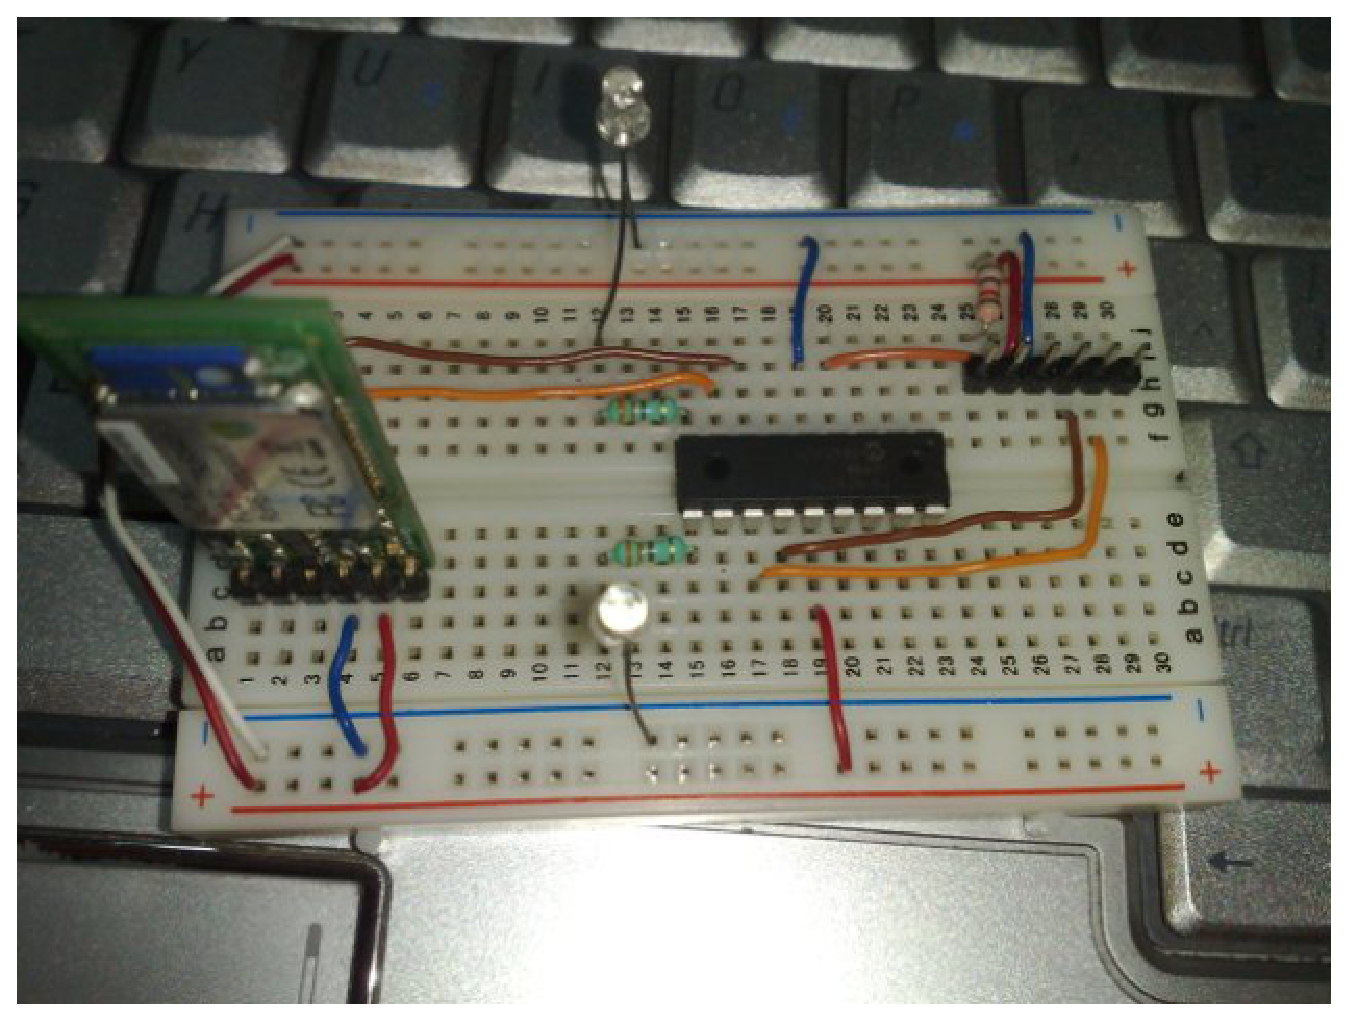
\includegraphics[width=0.4\textwidth]{images/imagensinexplicar.eps}
        \caption{\footnotesize{Circuito microcontrolador-bluetooth}}
        \label{fig1_101}
\end{figure}

En general, si ustedes desconocen el tema tendrán una idea muy vaga respecto a la descripción de la imagen que se muestra. Para dejar clara la explicación de una imagen, la descripción puede realizarse como se muestra a continuación:

\emph{En la figura \ref{fig1_102} se muestra el circuito cableado para realizar la comunicación utilizando el protocolo de comunicación \textbf{bluetooth}. Este se encuentra basado en el uso de un microcontrolador y un dispositivo transceptor bluetooth. Para evitar posibles problemas de conexión o daño en el circuito integrado  microcontrolador se utilizó el sistema de programación ICSP para realizar la programación del mismo conectado a través de una tira de pines.}

\begin{figure}[!htbp]
        \centering
        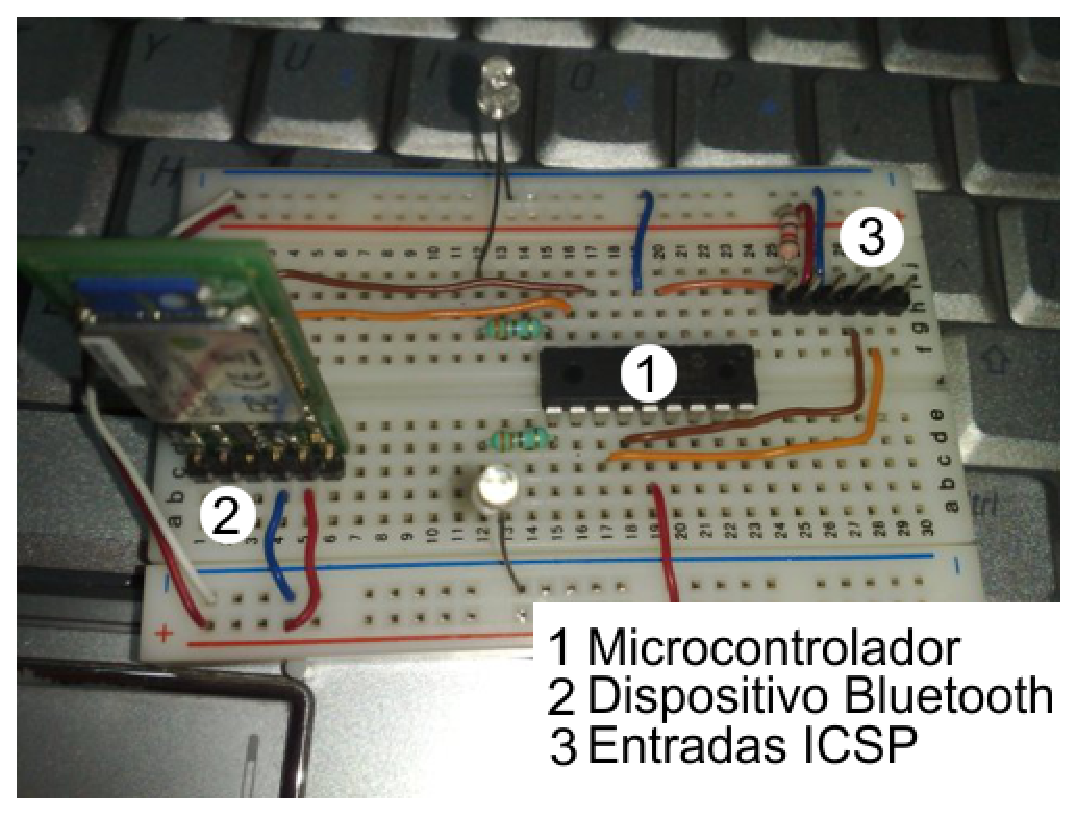
\includegraphics[width=0.4\textwidth]{images/imagenexplicada.eps}
        \caption{\footnotesize{Circuito microcontrolador-bluetooth}}
        \label{fig1_102}
\end{figure}

\subsubsection{Diagramas}

Los diagramas son formas gráficas para explicar algún procedimiento, algoritmo ó conexiones. Estos son útiles para resumir grandes cantidades de información mediante el uso de bloques, flechas y un poco de texto. Los diagramas son una de las herramientas de diseño más importantes en ingeniería, pues son fáciles de construir y fáciles de interpretar cuando están bien diseñados.

\begin{figure}[!htbp]
        \centering
        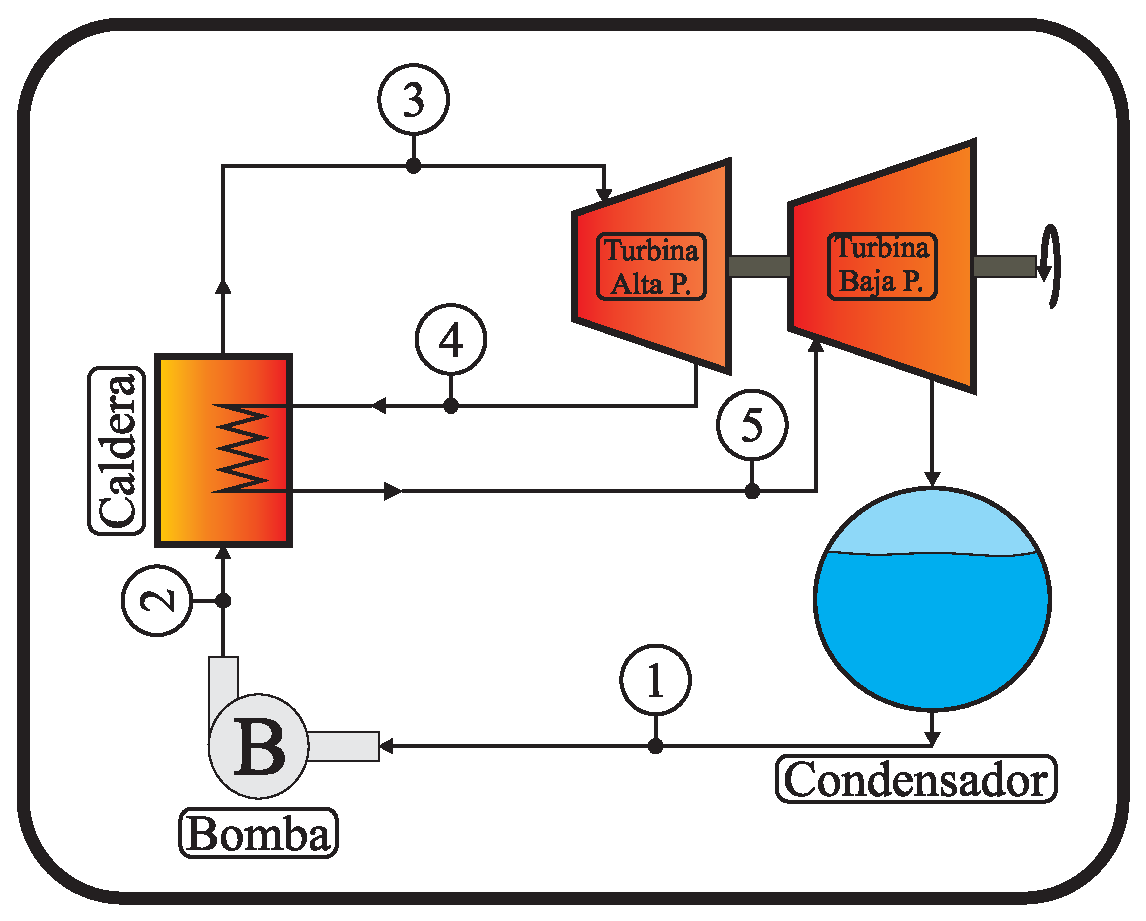
\includegraphics[width=0.4\textwidth]{images/rankine_rec.eps}
        \caption{\footnotesize{Ciclo Rankine con recalentamiento}}
        \label{fig1_103}
\end{figure}


Por ejemplo, en la figura \ref{fig1_103} se muestra un diagrama que explica el ciclo Rankine con recalentamiento. Como se observa las flechas del diagrama indican el sentido de flujo del vapor y la conexión entre los diferentes elementos que conforman el ciclo. De igual manera en el diagrama se hacen notar puntos clave (identificados mediante el uso de un punto de prueba denotado por un número) que sirven para hacer ampliar la explicación del diagrama.

\subsubsection{Gráficas}

Es común el uso de gráficas para simplificar grandes cantidades de datos, o para mostrar el comportamiento de un fenómeno. Las gráficas que se incluyan deben contener la suficiente información para que el usuario pueda, mediante un breve análisis, extraer información concreta de las mismas. Para lograr este objetivo es necesario incluir en las gráficas todas las cotas necesarias respecto a la información que se presenta. Por ejemplo, la gráficas de la figura  \ref{fig1_107} contiene etiquetas para los ejes coordenados que indican el nombre de la variable a la que hace referencia la gráfica, de igual manera contiene un cuadro de texto en el cuál se indica el nombre de cada una de las gráficas mostradas en la figura, y finalmente, la figura también tiene un nombre que indica que representa la gráfica en conjunto. Con la información proporcionada el lector tendrá una idea más clara de los resultados presentados, y le será fácil realizar un análisis de la misma y llegar a una conclusión.

\begin{figure}[!htbp]
        \centering
        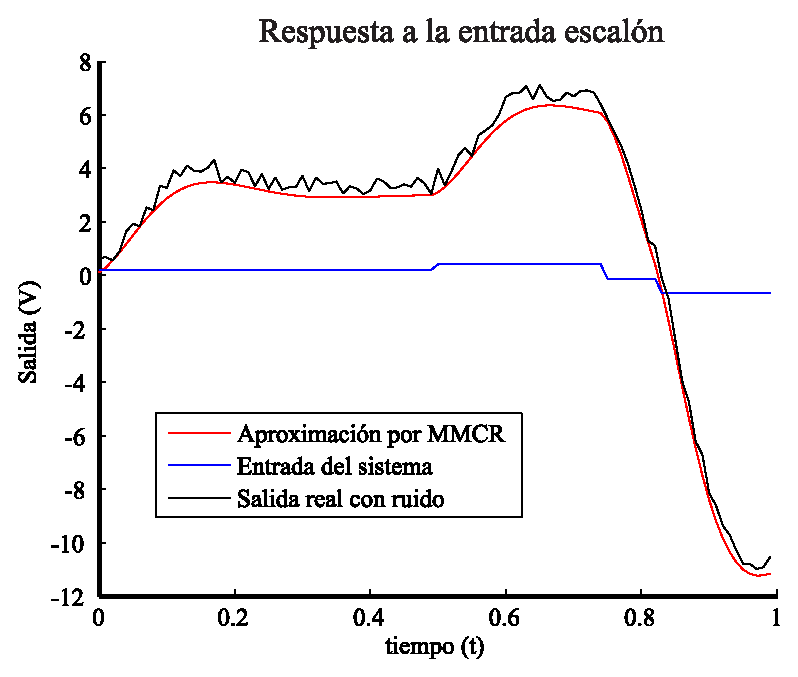
\includegraphics[width=0.4\textwidth]{images/grafica.eps}
        \caption{\footnotesize{Aproximación por mínimos cuadrados recursivos}}
        \label{fig1_107}
\end{figure}

Cuando se cuenta con una gran cantidad de datos, es totalmente recomendable utilizar una gráfica para mostrar resultados y realizar análisis, colocar un exceso de datos en una tabla hace casi imposible analizar los datos que en esta se presenten.


\begin{figure}[!htbp]
        \centering
        \includegraphics[width=0.4\textwidth]{images/error.eps}
        \caption{\footnotesize{Análisis del error}}
        \label{figuram99}
\end{figure}

Otro ejemplo se muestra en la figura \ref{figuram99}, el la cuál se presenta el análisis para el error obtenido al realizar una aproximación mediante el uso de redes neuronales.
